\subsection{Win32 PE}

\acs{PE} \IFRU{это формат исполняемых файлов, принятый в Windows}{is a executable file format used in
Windows}.

\IFRU{Разница между .exe, .dll, и .sys в том, что у .exe и .sys обычно нет экспортов, только импорты}
{The difference between .exe, .dll and .sys is that .exe and .sys usually does not have exports, only imports}.

\IFRU{У \ac{DLL}, как и у всех PE-файлов, есть точка входа (\ac{OEP})
(там располагается ф-ция DllMain()), но обычно эта ф-ция ничего не делает.}
{A \ac{DLL}, just as any other PE-file, has entry point (\ac{OEP}) (the function DllMain() is located at it) 
but usually this function does nothing.}

.sys \IFRU{это обычно драйвера устройств}{is usually device driver}.

\IFRU{Для драйверов, Windows требует чтобы контрольная сумма в PE-файле была проставлена
и была верной}
{As of drivers, Windows require that checksum is present in PE-file and must be correct}
\footnote{\IFRU{Например}{For example}, Hiew\ref{Hiew} \IFRU{умеет её подсчитывать}{can calculate it}}.

\IFRU{А начиная с}{Starting at} Windows Vista, 
\IFRU{PE-файлы-драйвера должны быть также подписаны при помощи электронной подписи, 
иначе они не будут загружаться.}
{driver PE-files must be also signed by digital signature. It will fail to load without signature.}

\index{MS-DOS}
\IFRU{В начале всякого PE-файла есть крохотная DOS-программа,
выводящая на консоль сообщение вроде}{Any PE-file begins with tiny DOS-program, printing a
message like} ``This program cannot be run in DOS mode.'' --- 
\IFRU{если запустить эту программу в DOS либо Windows 3.1, выведется это сообщение}
{if to run this program in DOS or Windows 3.1, this message will be printed}.

\subsubsection{\IFRU{Терминология}{Terminology}}

\begin{itemize}
\item
\IFRU{Модуль}{Module} --- \IFRU{это отдельный файл}{is a separate file}, .exe \OrENRU .dll.

\item
\IFRU{Процесс}{Process} --- \IFRU{это некая загруженная в память и работающая программа}{a program
loaded into memory and running}.
\IFRU{Как правило состоит из одного .exe-файла и массы .dll-файлов}{Commonly consisting of 
one .exe-file and bunch of .dll-files}.

\item
\IFRU{Память процесса}{Process memory} --- \IFRU{память с которой работает процесс}{the memory a process
works with}.
\IFRU{У каждого процесса --- своя}{Each process has its own}.
\IFRU{Там обычно имеются загруженные модули, память стека, кучи (heap), итд}{There can usually be 
loaded modules, memory of the stack, heap(s), etc}.

\item
\ac{VA} --- \IFRU{это адрес, который будет использоваться в самой программе}{is address which will
be used in program}.

\item
\IFRU{Базовый адрес}{Base address} --- \IFRU{это адрес, по которому модуль будет загружен 
в пространство процесса}{is the address within a process memory at which a module will be loaded}.

\item
\ac{RVA} --- \IFRU{это}{is a} \ac{VA}-\IFRU{адрес минус базовый адрес}{address minus base address}.
\IFRU{Многие адреса в таблицах PE-файла используют именно}{Many addresses in PE-file tables
uses exactly} \ac{RVA}-\IFRU{адреса}{addresses}.

\item
\ac{IAT} --- \IFRU{самая главная таблица описывающая импорты}{most important table which describes
imports}\footnote{\cite{Pietrek1}}.
\end{itemize}

\subsubsection{\IFRU{Базовый адрес}{Base address}}

\IFRU{Дело в том что несколько авторов модулей могут готовить DLL-файлы для других, и нет возможности договориться о том, какие адреса и кому будут отведены.}
{The fact is that several module authors may prepare DLL-files for others and there are no possibility
to reach agreement, which addresses will be assigned to whose modules.}

\IFRU{Поэтому, если у двух необходимых для загрузки процесса DLL одинаковые базовые адреса,
одна из них будет загружена по этому базовому адресу, 
а вторая ~--- по другому свободному месту в памяти процесса, и все виртуальные адреса
во второй DLL будут скорректированы.}
{So that is why if two necessary for process loading DLLs has the same base addresses,
one of which will be loaded at this base address, and another ~--- at the other spare space in process memory,
and each virtual addresses in the second DLL will be corrected.} \\
\\
\IFRU{Очень часто линкер в}{Often, linker in} \ac{MSVC} \IFRU{генерирует .exe-файлы с базовым адресом}
{generates an .exe-files with the base address} \TT{0x400000},
\IFRU{и с секцией кода начинающейся с}{and with the code section started at} \TT{0x401000}.
\IFRU{Это значит что}{This mean} \ac{RVA} \IFRU{начала секции кода ~---}{of code section begin is} \TT{0x1000}.
\IFRU{А \ac{DLL} часто генерируются этим линкером с базовым адресом}
{DLLs are often generated by this linked with the base address} \TT{0x10000000}
\footnote{\IFRU{Это можно изменять опцией /BASE в линкере}{This can be changed by /BASE linker option}}.

\index{ASLR}
\IFRU{Помимо всего прочего, есть еще одна причина намеренно загружать модули по разным адресам, а точнее, 
по случайным}{There are also one more reason to load modules at different base addresses, rather at random ones}.

\IFRU{Это}{It is} \ac{ASLR}
\footnote{\IFRU{\url{https://ru.wikipedia.org/wiki/Address_Space_Layout_Randomization}}
{\url{https://en.wikipedia.org/wiki/Address_space_layout_randomization}}}.

\IFRU{Дело в том, что некий шеллкод, пытающийся исполниться на зараженной системе, 
должен вызывать какие-то системные ф-ции}{The fact is that a shellcode trying to be executed on a compromised
system must call a system functions}.

\IFRU{И в старых}{In older} \ac{OS} (\IFRU{в линейке Windows NT: до}{in Windows NT line: before} Windows Vista),
\IFRU{системные}{system} DLL (\IFRU{такие как}{like} kernel32.dll, user32.dll) \IFRU{загружались все время
по одним и тем же адресам}{were always loaded at the known addresses}, 
\IFRU{а если еще и вспомнить, что версии этих DLL редко менялись}{and also if to recall
that its versions were rarely changed}, \IFRU{то адреса отдельных
ф-ций, можно сказать, фиксированы и шеллкод может вызывать их напрямую}{an addresses of functions were
fixed and shellcode can call it directly}.

\IFRU{Чтобы избежать этого, методика}{In order to avoid this,} \ac{ASLR}
\IFRU{загружает и вашу программу, и все модули ей необходимые, по случайным адресам, разным при каждом запуске}
{method loads your program and all modules it needs at random base addresses, each time different}.

\subsubsection{Subsystem}

Имеется также поле subsystem, обычно это native (.sys-драйвер), console (консольное приложение) или \ac{GUI}
(не консольное).

\subsubsection{\IFRU{Версия ОС}{OS version}}

\IFRU{В PE-файле имеется минимальный номер версии Windows, необходимый для загрузки модуля.}
{A PE-file also has minimal Windows version needed in order to load it.}
\IFRU{Соответствие номеров версий в файле и кодовых наименований Windows, можно посмотреть}
{The table of version numbers stored in PE-file and corresponding Windows codenames is}
\href{https://en.wikipedia.org/wiki/Windows_NT#Releases}{\IFRU{здесь}{here}}.

\IFRU{Например}{For example}, \ac{MSVC} 2005 \IFRU{еще компилирует .exe-файлы запускающиеся на}{compiles
.exe-files running on} Windows NT4 (\IFRU{версия}{version} 4.00),
\IFRU{а вот}{but} \ac{MSVC} 2008 \IFRU{уже нет}{is not} 
(\IFRU{генерируемые файлы имеют версию}{files generated has version} 5.00, 
\IFRU{для запуска необходима как минимум Windows 2000}{at least Windows 2000 is needed to run them}).

\ac{MSVC} 2012 \IFRU{по умолчанию генерирует .exe-файлы версии}{by default generates .exe-files of version} 6.00, 
\IFRU{для запуска нужна как минимум Windows Vista}{targeting at least Windows Vista}, \IFRU{хотя}{however, by} 
\href{http://blogs.msdn.com/b/vcblog/archive/2012/10/08/10357555.aspx}{\IFRU{изменив настройки компиляции}
{by changing compiler's options}}, 
\IFRU{можно заставить генерировать и под Windows XP}{it is possible to force it to compile for Windows XP}.

\subsubsection{\IFRU{Секции}{Sections}}

\IFRU{Разделение на секции присутствует, по видимому, во всех форматах исполняемых файлов}{Division by sections,
as it seems, are present in all execuable file formats}.

\IFRU{Сделано это для того, чтобы отделить код от данных, а данные ~--- от константных данных.}
{It is done in order to separate code from data, and data ~--- from constant data.}

\begin{itemize}
\item
\IFRU{На секции кода будет стоять флаг}{There will be flag} 
\IT{IMAGE\_SCN\_CNT\_CODE} \OrENRU \IT{IMAGE\_SCN\_MEM\_EXECUTE}\IFRU{}{ on code section}
~--- \IFRU{это исполняемый код}{this is executable code}.

\item
\IFRU{На секции данных}{On data section} ~--- \IFRU{флаги }{}\IT{IMAGE\_SCN\_CNT\_INITIALIZED\_DATA}, 
\IT{IMAGE\_SCN\_MEM\_READ} \AndENRU \IT{IMAGE\_SCN\_MEM\_WRITE}\IFRU{}{ flags}.

\item
\IFRU{На пустой секции с неинициализированными данными}{On an empty section with uninitialized data} ~--- 
\IT{IMAGE\_SCN\_CNT\_UNINITIALIZED\_DATA}, \IT{IMAGE\_SCN\_MEM\_READ} \AndENRU \IT{IMAGE\_SCN\_MEM\_WRITE}.

\item
\IFRU{А на секции с константными данными, то есть, защищенными от записи}{On a constant data section, in other words,
protected from writing}, \IFRU{могут быть флаги}{there are may be flags} \\
\IT{IMAGE\_SCN\_CNT\_INITIALIZED\_DATA} \AndENRU \IT{IMAGE\_SCN\_MEM\_READ} \IFRU{без}{without} \IT{IMAGE\_SCN\_MEM\_WRITE}. 
\IFRU{Если попытаться записать что-то в эту секцию, процесс упадет}{A process will crash if it would try to write to this
section}.
\end{itemize}

\IFRU{В PE-файле можно задавать название для секции, но это не важно}{Each section in PE-file may have a name, however,
it is not very important}.
\IFRU{Часто (но не всегда)}{Often (but not always)} \IFRU{секция кода называется}{code section have the name} \TT{.text}, 
\IFRU{секция данных}{data section} --- \TT{.data}, \IFRU{константных данных}{constant data section} --- \TT{.rdata} 
\IT{(readable data)}.
\IFRU{Еще популярные имена секций}{Other popular section names are}: 
\TT{.idata} (\IFRU{секция импортов}{imports section}),
\TT{.edata} (\IFRU{секция экспортов}{exports section}),
\TT{.reloc} (\IFRU{секция релоков}{relocs section}),
\TT{.bss} (\IFRU{неинициализированные данные}{uninitialized data (\ac{BSS})}),
\TT{.tls} ~--- thread local storage (\ac{TLS}),
\TT{.rsrc} (\IFRU{ресурсы}{resources}).

\IFRU{Запаковщики/зашифровщики PE-файлов часто затирают имена секций, или меняют на свои}
{PE-file packers/encryptors are often garble section names or replacing names to their own}.

\IFRU{В \ac{MSVC} можно объявлять данные в произвольно названной секции}
{\ac{MSVC} allows to declare data in arbitrarily named section}
\footnote{\url{http://msdn.microsoft.com/en-us/library/windows/desktop/cc307397.aspx}}.

\IFRU{Некоторые компиляторы и линкеры могут добавлять также секцию с отладочными символами 
и вообще отладочной информацией}
{Some compilers and linkers can add a section with debugging symbols and other debugging information}
(\IFRU{например}{for example}, MinGW).
\index{PDB}
\IFRU{Хотя это не так в современных версиях}{However it is not so in modern versions of} \ac{MSVC} 
(\IFRU{там принято отладочную информацию сохранять в отдельных PDB-файлах}
{a separate PDB-files are used there for this purpose}).

\subsubsection{\IFRU{Релоки}{Relocations (relocs)}}

\IFRU{Так же известны как FIXUP-ы}{\ac{AKA} FIXUP-s}.

\IFRU{Это также присутствует почти во всех форматах загружаемых и исполняемых файлов}
{This is also present in almost all executable file formats}
\footnote{\IFRU{Даже .exe-файлы в}{Even .exe-files in} MS-DOS}.

\IFRU{Как видно, модули могут загружаться по другим базовым адресам,
но как же тогда работать с глобальными переменными, например?}
{Obviously, modules are can be loaded on different base addresses, but how to work with global variables,
for example?}
\IFRU{Ведь нужно обращаться к ним по адресу}{They must be accessed by an address}.
\IFRU{Одно из решений это}{One solution is} \PICcode\ref{sec:PIC}. 
\IFRU{Но это далеко не всегда удобно}{But it is not always suitable}.

\IFRU{Поэтому имеется таблица релоков. 
Там просто перечислены адреса мест в модуле подлежащими коррекции при загрузке
по другому базовому адресу.}
{That is why relocations table is present.
The addresses of points needs to be corrected in case of loading on another base address 
are just enumerated in the table.}

\IFRU{Например, по}{For example, there are a global variable at the address}
\TT{0x410000} 
\IFRU{лежит некая глобальная переменная, и вот как обеспечивается её чтение}
{and that is how it is accessed}:

\begin{lstlisting}
A1 00 00 41 00         mov         eax,[000410000]
\end{lstlisting}

\IFRU{Базовый адрес модуля}{Base address of module is} \TT{0x400000},
\IFRU{а }{}\ac{RVA} \IFRU{глобальной переменной}{of global variable is} \TT{0x10000}.

\IFRU{Если загружать модуль по базовому адресу}{If the module is loading on the base address}
\TT{0x500000}, \IFRU{нужно чтобы адрес этой переменной в этой инструкции стал}{the factual address
of the global variable must be} \TT{0x510000}.

\IFRU{Как видно, адрес переменной закодирован в самой инструкции}
{As we can see, address of variable is encoded in the instruction} \TT{MOV}, 
\IFRU{после байта}{after the byte} \TT{0xA1}.

\IFRU{Поэтому адрес четырех байт}{That is why address of 4 bytes}, \IFRU{после}{after} \TT{0xA1},
\IFRU{записыватся в таблицу релоков}{is written into relocs table}.

\IFRU{Если модуль загружается по другому базовому адресу},
\IFRU{загрузчик \ac{OS} обходит все адреса в таблице}{\ac{OS}-loader enumerates all addresses in table}, 
\IFRU{находит каждое 32-битное слово по этому адресу}{finds each 32-bit word on that address},
\IFRU{отнимает от него настоящий, оригинальный базовый адрес}{subtracts real, original base address of it}
(\IFRU{в итоге получается}{we getting} \ac{RVA}\IFRU{}{ here}),
\IFRU{и прибавляет к нему новый базовый адрес}{and adds new base address to it}.


\IFRU{А если модуль загружается по своему оригинальному базовому адресу, ничего не происходит}
{If module is loading on original base address, nothing happens}.

\IFRU{Так можно обходиться со всеми глобальными переменными}{All global variables may be treated like that}.

\IFRU{Релоки могут быть разных типов}{Relocs may have various types}, 
\IFRU{однако в Windows для x86-процессоров, тип обычно}
{however, in Windows, for x86 processors, the type is usually} \\
\IT{IMAGE\_REL\_BASED\_HIGHLOW}.

\subsubsection{\IFRU{Экспорты и импорты}{Exports and imports}}

\IFRU{Как известно}{As all we know}, 
\IFRU{любая исполняемая программа должна как-то пользоваться сервисами \ac{OS} и прочими DLL-библиотеками}
{any executable program must use \ac{OS} services and other DLL-libraries somehow}.

\IFRU{Можно сказать, что нужно связывать функции из одного модуля (обычно DLL) и места их вызовов в 
другом модуле (.exe-файл или другая DLL)}
{It can be said, functions from one module (usually DLL) must be connected somehow to a points of their
calls in other module (.exe-file or another DLL)}.

\IFRU{Для этого, у каждой DLL есть ``экспорты'', это таблица ф-ций плюс их адреса в модуле}
{Each DLL has ``exports'' for this, this is table of functions plus its addresses in a module}.

\IFRU{А у .exe-файла, либо DLL, есть ``импорты'', (\ac{IAT}) это таблица ф-ций требующихся для исполнения 
включая список имен DLL-файлов}
{Each .exe-file or DLL has ``imports'', (\ac{IAT}) this is a table of functions it needs for execution including
list of DLL filenames}.

\IFRU{Загрузчик \ac{OS}, после загрузки основного .exe-файла, проходит по \ac{IAT}:
загружает дополнительные DLL-файлы, 
находит имена ф-ций среди экспортов в DLL и прописывает их адреса в \ac{IAT} в головном .exe-модуле}
{After loading main .exe-file, \ac{OS}-loader, processes \ac{IAT}: 
it loads additional DLL-files, finds function names
among DLL exports and writes their addresses down in an \ac{IAT} of main .exe-module}.

\IFRU{Как видно, во время загрузки, загрузчику нужно много сравнивать одни имена ф-ций с другими, а сравнение строк
это не очень быстрая процедура, так что,
имеется также поддержка ``ординалов'' или 
``hint''-ов, это когда в таблице импортов проставлены номера ф-ций вместо их имен}
{As we can notice, during loading, loader must compare a lot of function names, but strings comparison is not a very
fast procedure, so, there are support of ``ordinals'' or ``hints'',
that is a function numbers stored in the table instead of their names}.

\IFRU{Так их быстрее находить в загружаемой DLL}{That is how they can be located faster in loading DLL}.
\IFRU{В таблице экспортов ординалы присутствуют всегда}{Ordinals are always present in ``export'' table}.

\index{MFC}
\IFRU{К примеру}{For example}, \IFRU{программы использующие библиотеки}{program using} 
\ac{MFC}\IFRU{, обычно загружают mfc*.dll по ординалам}{ library usually loads mfc*.dll by ordinals},
\IFRU{и в таких программах, в \ac{IAT}, нет имен ф-ций \ac{MFC}}
{and in such programs there are no \ac{MFC} function names in \ac{IAT}}.

\IFRU{При загрузке такой программы в \IDA, она спросит у вас путь к файлу mfc*.dll,
чтобы установить имена ф-ций}{While loading such program in \IDA, it will asks for a path to mfs*.dll files,
in order to determine function names}.
\IFRU{Если в \IDA не указать путь к этой DLL, то вместо имен ф-ций будет что-то вроде}
{If not to tell \IDA path to this DLL, there are will something like}
\IT{mfc80\_123}\IFRU{}{ instead of function names}.

\paragraph{\IFRU{Секция импортов}{Imports section}}

\IFRU{Под \ac{IAT} и всё что с ней связано иногда отводится отдельная секция (с названием вроде \TT{.idata}),
но это не обязательно}
{Often a separate section is allocated for \ac{IAT} table and everything related to it (with name like \TT{.idata}),
however, it is not a strict rule}.

\IFRU{Импорты это запутанная тема еще и из-за терминологической путанницы. Попробуем собрать всё в одно место.}
{Imports is also confusing subject because of terminological mess. Let's try to collect all information in one place.}

\begin{figure}[ht!]
\centering
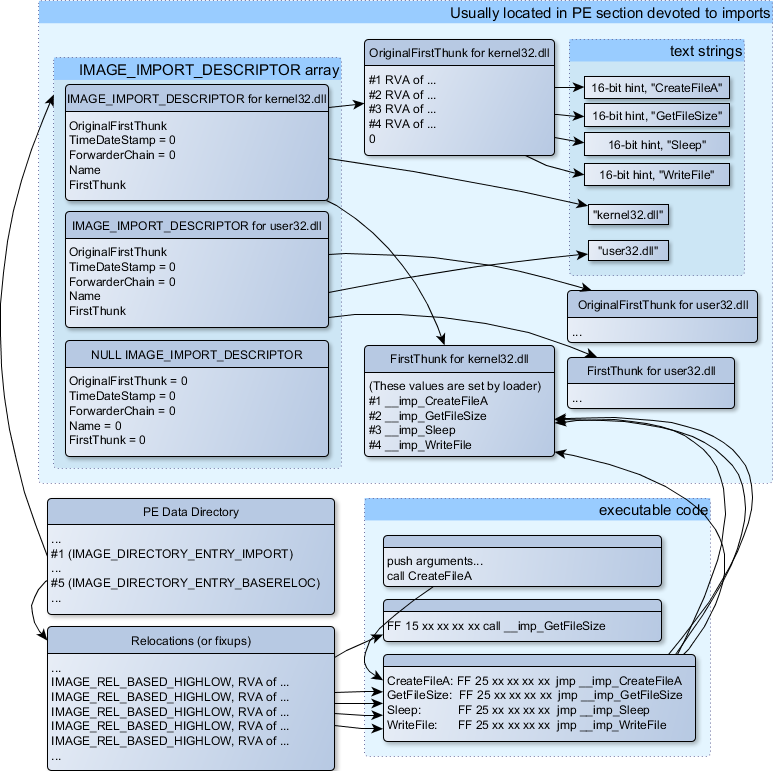
\includegraphics[scale=0.66]{OS-specific/PE/unnamed0.png}
\caption{\IFRU{схема, объеденяющая все структуры в PE-файлы, связанные с импортами}
{The scheme, uniting all PE-file structures related to imports}}
\end{figure}

\IFRU{Самая главная структура, это массив}{Main structure is the array of} \IT{IMAGE\_IMPORT\_DESCRIPTOR}.
\IFRU{Каждый элемент на каждую импортируемую DLL}{Each element for each DLL being imported}.

\IFRU{У каждого элемента есть}{Each element holds} \ac{RVA}-\IFRU{адрес}{address} 
\IFRU{текстовой строки (имя DLL)}{of text string (DLL name)} (\IT{Name}).

\IT{OriginalFirstThink} \IFRU{это}{is a} \ac{RVA}-\IFRU{адрес}{address} \IFRU{массива}{of array of} 
\ac{RVA}-\IFRU{адресов}{addresses},
\IFRU{каждый из которых указывает на текстовую строку где записано имя ф-ции}
{each of which points to the text string with function name}. 
\IFRU{Каждую строку предваряет 16-битное число}{Each string is prefixed by 16-bit integer} (``hint'') ~--- 
\IFRU{``ординал'' ф-ции}{``ordinal'' of function}.

\IFRU{Если при загрузке удается найти ф-цию по ординалу, тогда сравнение текстовых строк не будет происходить.
Массив оканчивается нулем}{While loading, if it is possible to find function by ordinal,
then strings comparison will not occur. Array is terminated by zero}.
\IFRU{Есть также указатель с названием}{There are also pointer with the name} \IT{FirstThunk},
\IFRU{это просто}{it is just} \ac{RVA}-\IFRU{адрес}{address} 
\IFRU{места, где загрузчик будет проставлять адреса найденных ф-ций}{of the place where loader will
write addresses of functions resolved}.

\IFRU{Места где загрузчик проставляет адреса, \IDA именует их так}{The points where
loader writes addresses, \IDA marks like}: \IT{\_\_imp\_CreateFileA}, \IFRU{итд}{etc}.

\IFRU{Есть по крайней мере два способа использовать адреса проставленные загрузчиком}
{There are at least two ways to use addresses written by loader}.

\begin{itemize}
\item
\IFRU{В коде будут просто инструкции вроде}{The code will have instructions like} 
\IT{call \_\_imp\_CreateFileA}, 
\IFRU{а так как, поле с адресом импортируемой ф-ции это как бы глобальная переменная}
{and since the field with the address of function imported is a global variable in some sense}, 
\IFRU{то в таблице релоков добавляется адрес (плюс 1 или 2) в инструкции \IT{call}}
{the address of \IT{call} instruction (plus 1 or 2) will be added to relocs table},
\IFRU{на случай если модуль будет загружен по другому базовому адресу}
{for the case if module will be loaded on different base address}.

\IFRU{Но как видно, это приводит к увеличению таблицы релоков}{But, obviously, this may enlarge
relocs table significantly}.
\IFRU{Ведь вызовов импортируемой ф-ции у вас в модуле может быть очень много}
{Because there are might be a lot of calls to imported functions in the module}.
\IFRU{К тому же, чем больше таблица релоков, тем дольше загрузка}
{Furthermore, large relocs table slowing down the process of module loading}.

\index{thunk-\IFRU{функции}{functions}}
\item
\IFRU{На каждую импортируемую ф-цию выделяется только один переход на импортируемую ф-цию используя
инструкцию \JMP плюс релок на эту инструкцию}
{For each imported function, there are only one jump allocated, using \JMP instruction 
plus reloc to this instruction}.
\IFRU{Такие места-``переходники'' называются также ``thunk''-ами}{Such points are also called ``thunks''}.
\IFRU{А все вызовы импортируемой ф-ции это просто инструкция \CALL на соответствующий ``thunk''}
{All calls to the imported functions are just \CALL instructions to the corresponding ``thunk''}.
\IFRU{В данном случае, дополнительные релоки не нужны, потому что эти CALL-ы имеют относительный адрес,
и корректировать их не надо}{In this case, additional relocs are not necessary because these CALL-s
has relative addresses, they are not to be corrected}.
\end{itemize}

\IFRU{Оба этих два метода могут комбинироваться}{Both of these methods can be combined}.
\IFRU{Вероятно, линкер создает отдельный ``thunk'', если вызовов слишком много, но по умолчанию --- не создает}
{Apparently, linker creates individual ``thunk'' if there are too many calls to the functions,
but by default it is not to be created}. \\
\\
\IFRU{Кстати, массив адресов ф-ций, на который указывает FirstThunk,
не обязательно может быть в секции \ac{IAT}}{By the way, an array of function addresses to which FirstThunk is
pointing is not necessary to be located in \ac{IAT} section}.
\IFRU{К примеру, я написал утилиту}{For example, I once wrote the}
PE\_add\_import\footnote{\url{http://yurichev.com/PE_add_import.html}} 
\IFRU{для добавления импорта в уже существующий .exe-файл}{utility for adding import to an existing .exe-file}.
\IFRU{На месте ф-ции, вместо которой вы хотите подставить вызов в другую DLL,
моя утилита вписывает такой код}{At the place of the function you want to substitute by call to another DLL,
the following code my utility writes}:

\begin{lstlisting}
MOV EAX, [yourdll.dll!function]
JMP EAX
\end{lstlisting}

\IFRU{При этом, FirstThunk указывает прямо на первую инструкцию.
Иными словами, загрузчик, загружая yourdll.dll, 
прописывает адрес ф-ции \IT{function} прямо в коде.}
{FirstThunk points to the first instruction. In other words, while loading yourdll.dll,
loader writes address of the \IT{function} function right in the code.}

\IFRU{Надо также отметить что обычно секция кода защищена от записи}{It also worth noting that
code section is usually write-protected}, \IFRU{так что, моя утилита
добавляет флаг}{so my utility adds} \IT{IMAGE\_SCN\_MEM\_WRITE} 
\IFRU{для секции кода. Иначе при загрузке такой программы, она упадет с ошибкой}
{flag for code section. Otherwise, the program will crash while loading with the error code}
5 (access denied). \\
\\
\IFRU{Может возникнуть вопрос: а что если я поставляю программу с набором DLL,
которые никогда не будут меняться, может как-то можно ускорить процесс загрузки?}
{One might ask: what if I supply a program with the DLL files set which are not supposed to change,
is it possible to speed up loading process?}

\IFRU{Да, можно прописать адреса импортируемых ф-ций в массивы FirstThunk зараннее}
{Yes, it is possible to write addresses of the functions to be imported into FirstThunk arrays in advance}.
\IFRU{Для этого в структуре}{The \IT{Timestamp} field is present in the} 
\IT{IMAGE\_IMPORT\_DESCRIPTOR} \IFRU{имеется поле \IT{Timestamp}{structure}.
\IFRU{И если там присутствует какое-то значение, то загрузчик сверяет это значение с датой-временем DLL-файла}
{If some value is present there, then loader compare this value with date-time of the DLL file}.
\IFRU{И если они равны, то загрузчик больше ничего не делает, и загрузка будет происходить быстрее}
{If the values are equal to each other, then the loader is not do anything, and loading process will be faster}.\IFRU{Это называется}{This is what called} ``old-style binding''
\footnote{\url{http://blogs.msdn.com/b/oldnewthing/archive/2010/03/18/9980802.aspx}.
\IFRU{Существует также}{There is also} ``new-style binding'',
\IFRU{про него напишу позже}{I will write about it in future}}.
\IFRU{В Windows SDK для этого имеется утилита BIND.EXE}
{There is the BIND.EXE utility in Windows SDK for this}.
\IFRU{Для ускорения загрузки вашей программы}{For speeding up of loading of your program}, 
Matt Pietrek \In \cite{Pietrek1}, \IFRU{предлагает делать binding сразу после инсталляции
вашей программы на компьютере конечного пользователя}{offers to do binding shortly after your program
installation on the computer of the end user}. \\
\\
\IFRU{Запаковщики/зашифровщики PE-файлов могут также сжимать/шифровать \ac{IAT}}
{PE-files packers/encryptors may also comporess/encrypt \ac{IAT}}.
\IFRU{В этом случае, загрузчик Windows, конечно же, не загрузит все нужные DLL}
{In this case, Windows loader, of course, will not load all necessary DLLs}.
\IFRU{Поэтому распаковщик/расшифровщик делает это сам, при помощи вызовов}
{Therefore, packer/encryptor do this on its own, with the help of} 
\IT{LoadLibrary()} \AndENRU \IT{GetProcAddress()}\IFRU{}{ functions}. \\
\\
\IFRU{В стандартных DLL входящих в состав Windows, часто, \ac{IAT} находится в самом начале PE-файла}
{In the standard DLLs from Windows installation, often, \ac{IAT} is located right in the beginning of PE-file}.
\IFRU{Возможно это для оптимизации}{Supposedly, it is done for optimization}.
\IFRU{Ведь .exe-файл при загрузке не загружается в память весь 
(вспомните что инсталляторы огромного размера подозрительно быстро запускаются), он ``мапится'' (map), 
и подгружается в память частями по мере обращения к этой памяти.}
{While loading, .exe file is not loaded into memory as a whole (recall huge install programs which are
started suspiciously fast), it is ``mapped'', and loaded into memory by parts as they are accessed.}
\IFRU{И возможно в Microsoft решили что так будет быстрее}
{Probably, Microsoft developers decided it will be faster}.

\subsubsection{\IFRU{Ресурсы}{Resources}}

Ресурсы в PE-файле это набор иконок, картинок, текстовых строк, описаний диалогов.
Возможно, их в свое время решили выделить в отдельное место, чтобы все эти вещи были мультиязычными,
и было проще выбирать текст или картинку того языка, который установлен в \ac{OS}. \\
\\
В качестве побочного эффекта, их легко редактировать и сохранять обратно, даже не обладая специальными знаниями,
например, редактором ResHack\ref{ResHack}.

\subsubsection{.NET}

\index{.NET}
Программы на .NET компилируются не в машинный код, а в свой собственный байткод.
Собственно, в .exe-файлы байткод вместо обычного кода, однако, точка входа (\ac{OEP}) 
указывает на крохотный фрагмент x86-кода:

\begin{lstlisting}
jmp         mscoree.dll!_CorExeMain
\end{lstlisting}

А в mscoree.dll и находится .NET-загрузчик, который уже сам будет работать с PE-файлом.

\index{TLS}
\subsubsection{TLS}

Эта секция содержит в себе инициализированные данные для \ac{TLS}\ref{TLS} (если нужно).
При старте нового треда, его \ac{TLS}-данные инициализируются данными из этой секции. \\
\\
Помимо всего прочего, спецификация PE-файла предусматривает инициализацию \ac{TLS}-секции, т.н., TLS callbacks.
Если они присутствуют, то они будут вызваны перед тем как передать управление на точку входа (\ac{OEP}).
Это широко используется запаковщиками/защифровщиками PE-файлов.

\subsubsection{Инструменты}

\begin{itemize}
\item
\index{objdump}
\index{cygwin}
objdump (из cygwin) для вывода всех структур PE-файла

\item
Hiew\ref{Hiew} как редактор

\item
pefile --- Python-библиотека для работы с PE-файлами\footnote{\url{https://code.google.com/p/pefile/}}

\item
\label{ResHack}
ResHack \acs{AKA} Resource Hacker --- редактор ресурсов\footnote{\url{http://www.angusj.com/resourcehacker/}}
\end{itemize}

\subsubsection{Further reading}

% FIXME: bibliography per chapter or section
\begin{itemize}
\item
Daniel Pistelli --- The .NET File Format \footnote{\url{http://www.codeproject.com/Articles/12585/The-NET-File-Format}}
\end{itemize}

